\begin{answer}
\begin{figure}[H]
    \centering
    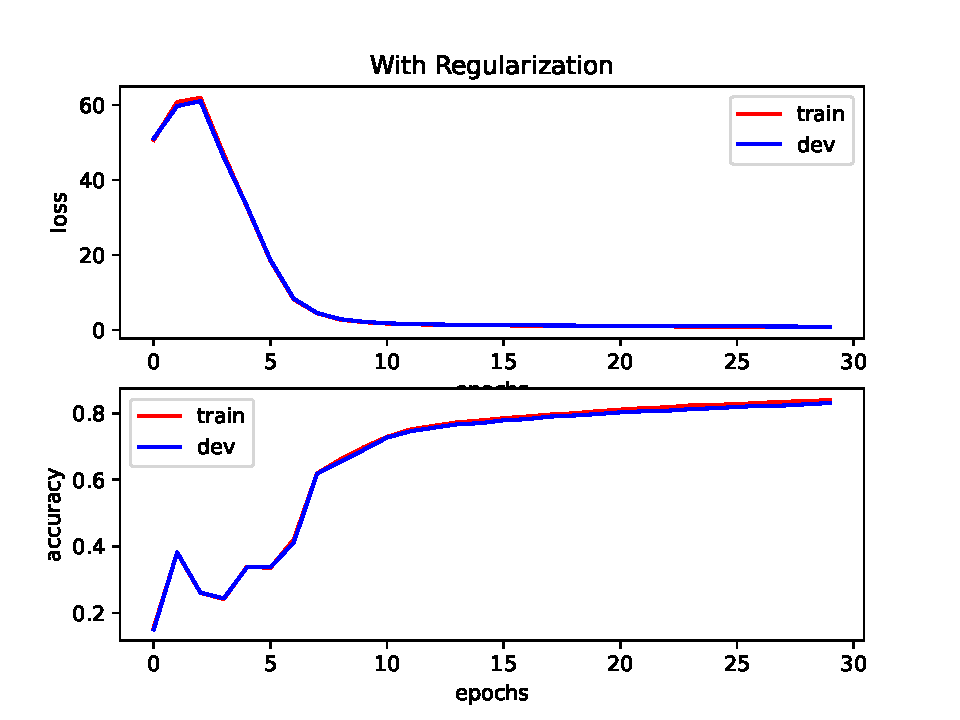
\includegraphics[width=0.5\linewidth]{regularized.pdf}
    \caption{Regularization}
    \label{fig:enter-label}
\end{figure}

Observations

1. For model baseline, got accuracy: 0.928700, for model regularized, got accuracy: 0.967600, regularized model has better accuracy than baseline model

2. Although the training losses for regularized and unregularized are similar, the dev loss of the model with regularization is significantly lower, and the blue line follows more closely with the red line, meaning when using dev, regularized model behaves more similarly with training.

3. Base on 1 and 2, we conclude that the performance on dev is a good indicator of the actual test data - lower loss on dev usually means better performance(accuracy) on real test data
\end{answer}
   
  
